% !TEX root = ../latexnote.tex
\chapter{参考文献设置}\label{chap:ref}
\section{问题}

\subsection{不按出现顺序引用}\label{subsec:not-in-order}
\qaq{问题:}Latex中ACM-Reference-Format顺序与论文引用顺序不一致

\qaq{解决方法:}修改\textcolor{red}{\lstinline{ACM-Reference-Format.bst}}文件,将大写SORT注释掉,一共两处。

\subsection{作者年份引用设置仅年份超链接}\label{subsec:year-only}
\qaq{问题:}Latex中采用作者年份引用,默认作者和年份都出现超链接,设置仅年份出现超链接

\qaq{解决方法:}在\lstinline|\begin{document}|前加入如下代码:
\begin{lstlisting}
\makeatletter
% Patch case where name and year are separated by aysep
\patchcmd{\NAT@citex}
  {\@citea\NAT@hyper@{%
     \NAT@nmfmt{\NAT@nm}%
     \hyper@natlinkbreak{\NAT@aysep\NAT@spacechar}{\@citeb\@extra@b@citeb}%
     \NAT@date}}
  {\@citea\NAT@nmfmt{\NAT@nm}%
   \NAT@aysep\NAT@spacechar\NAT@hyper@{\NAT@date}}{}{}

% Patch case where name and year are separated by opening bracket
\patchcmd{\NAT@citex}
  {\@citea\NAT@hyper@{%
     \NAT@nmfmt{\NAT@nm}%
     \hyper@natlinkbreak{\NAT@spacechar\NAT@@open\if*#1*\else#1\NAT@spacechar\fi}%
       {\@citeb\@extra@b@citeb}%
     \NAT@date}}
  {\@citea\NAT@nmfmt{\NAT@nm}%
   \NAT@spacechar\NAT@@open\if*#1*\else#1\NAT@spacechar\fi\NAT@hyper@{\NAT@date}}
  {}{}

\makeatother
\end{lstlisting}

\subsection{作者年份引用设置et al为斜体}\label{subsec:et-al-italic}
\qaq{问题:}Latex中采用作者年份引用,设置et al为斜体

\qaq{解决方法:}在相应\textcolor{red}{\lstinline|.bst|}文件中将\textcolor{red}{\lstinline{et~al.}}修改为\textcolor{red}{\lstinline|\\textit{et~al.}|},不要修改\textcolor{red}{\lstinline{et al}}

\subsection{beamer参考文献断行}\label{subsec:beamer-ref-break}
\qaq{问题:}beamer参考文献断行显示,如图\ref{fig:beamer-ref}所示。
\begin{figure}[!h]
  \centering
  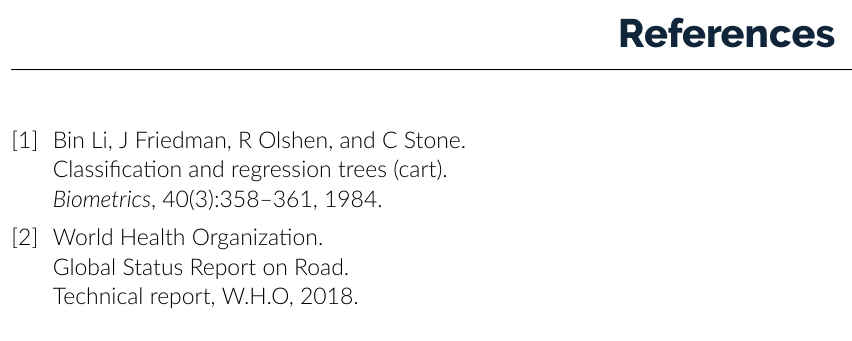
\includegraphics[width=0.8\textwidth]{figure/chap-ref/cankaowenxianduanhang.png}
  \caption{beamer参考文献断行显示}
  \label{fig:beamer-ref}
\end{figure}

\qaq{解决方法:}在导言区加入如下代码:
\begin{lstlisting}
  \setbeamertemplate{bibliography entry title}{}
  \setbeamertemplate{bibliography entry location}{}
  \setbeamertemplate{bibliography entry note}{}
\end{lstlisting}
\begin{figure}[!h]
  \centering
  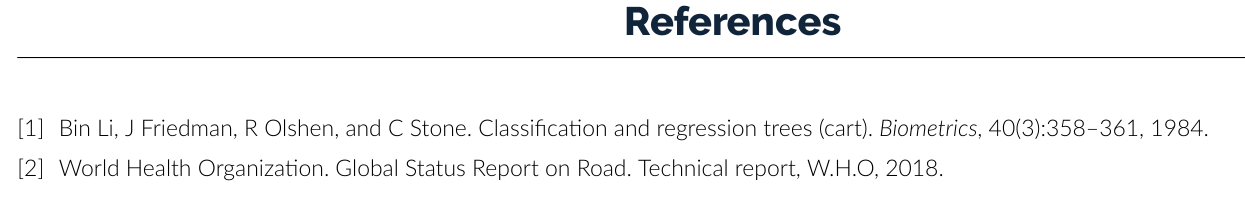
\includegraphics[width=0.8\textwidth]{figure/chap-ref/cankaowenxianduanhang1.png}
  \caption{beamer参考文献正常显示}
  \label{fig:beamer-ref1}
\end{figure}